\vspace{-0.5em}
\section{一种高效的同策略方法替代方案：半同策略蒸馏}
\vspace{-0.5em}

\label{sec:method}

\subsection{OPD的预备知识}

形式上，给定一个提示 $x \sim \mathcal{D}$，学生大模型 $\pi_\theta$ 会自回归地生成一个响应 $y=(y_1,\dots,y_T)$，访问前缀状态 $s_t=(x,y_{<t})$。其潜在的序列级目标是相对于固定教师 $\pi_T$ 的反向 $\mathrm{KL}(\pi_\theta(\cdot\mid x)\,\|\,\pi_T(\cdot\mid x))$。在实际操作中，一种常见的近似方法使用局部 token 级目标，仅在学生采样的 token 上评估教师-学生对数概率比，避免在每个位置进行全词表比较~\citep{lu2025onpolicydistillation, team2026kimi}。这得到了采样 token 目标：
\begin{equation}
\mathcal{L}_{OPD}(\theta)
=
\mathbb{E}_{x \sim \mathcal{D},\, y \sim \pi_\theta(\cdot \mid x)}
\left[
\sum_{t=1}^{T}
-A_t \cdot \log \pi_\theta(y_t \mid s_t)
\right],
\label{eq:opd}
\end{equation}
其中优势 $A_t
=
\log \pi_T(y_t \mid s_t)
-
\log \pi_\theta(y_t \mid s_t)$  在梯度中被视为常数。


如第~\ref{sec:intro} 节所述，近期工作已识别出同策略蒸馏（OPD）中的若干不良行为，例如重复的自我修正~\citep{luo2026demystifying,yang2026eos,fu2026revisiting}、对后续 token 的监督效果不佳~\citep{zhang2026fast,ziheng2026less}，以及一旦学生模型错误地确定方向后，监督变得不可靠~\citep{xu2026pass,jiang2026trajectory}。  
为研究蒸馏中同策略采样（on-policy sampling）的必要性，我们在第~\ref{sec:semi_opd_method} 节提出了一种简单替代方案——半同策略蒸馏（Semi-OPD）。




\begin{figure*}[t]
  \centering
  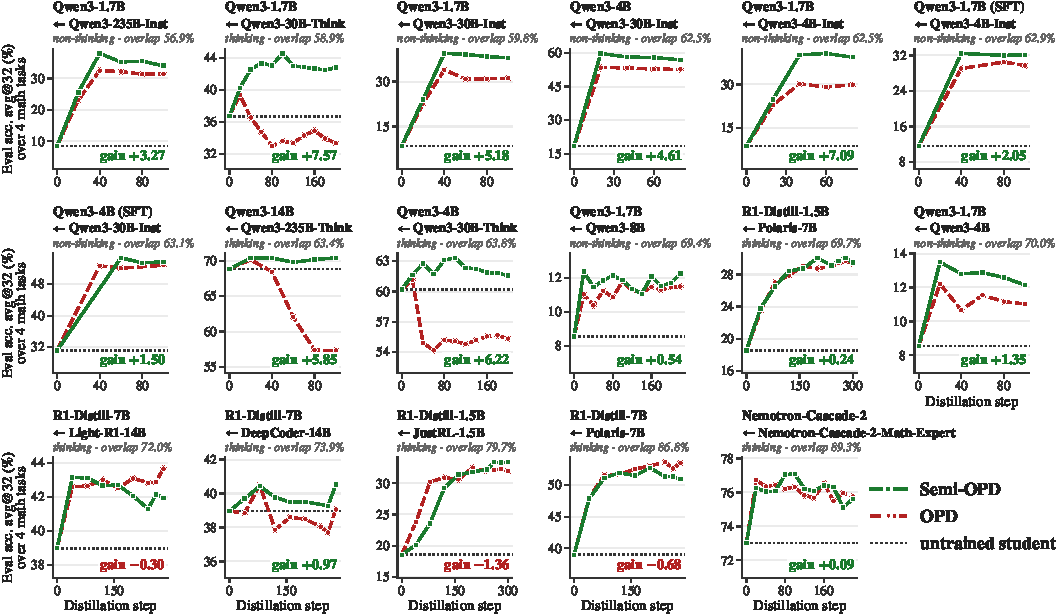
\includegraphics[width=0.95\linewidth]{fig3_allpairs.pdf}
\caption{
\textbf{半监督OPD与OPD在17组模型对中的对比。} 每个面板代表一组学生-教师模型对，其标题包含该对模型的初始前64重叠度。准确率以AIME 2024/2025/2026和HMMT 2026年2月的平均avg@32的均值衡量。每个面板中的数字是图~\ref{fig:overlap}a中绘制的增益，定义为两条曲线之间的面积除以训练周期。
  }
  \label{fig:allpairs}
  \vspace{-1em}
\end{figure*}




\subsection{半开放式配方}
\label{sec:semi_opd_method}

令 $\pi_0$ 表示初始学生，$\pi_\theta$ 表示正在被训练的学生。OPD 从当前学生 $y \sim \pi_\theta(\cdot \mid x)$ 中采样每个训练响应，因此训练数据会随着 $\theta$ 的更新而变化。半监督 OPD 则在训练开始前仅从初始学生中采样一次响应，
\begin{equation}
  \mathcal{D}_0 = \{(x_i, y_i)\}_{i=1}^{N}, \qquad y_i \sim \pi_0(\cdot \mid x_i).
\end{equation}
半OPD在整个训练过程中重复使用这个固定集合，以最小化与OPD相同的目標：
\begin{equation}
  \mathcal{L}_{\mathrm{\method}}(\theta)
  = \mathbb{E}_{(x,y) \sim \mathcal{D}_0}
  \Big[\sum_{t=1}^{T} -A_t \cdot \log \pi_\theta(y_t \mid s_t)\Big].
  \label{eq:semi-opd}
\end{equation}
尽管回溯轨迹是固定的，但学生模型的对数概率，以及由此产生的优势 $A_t$ ，是在每一步使用当前参数 $\theta$ 计算的，因此监督信号持续演化。



\noindent \textbf{Semi-OPD的训练效率。}
Semi-OPD将数据采集与最优化分离。我们首先从$\pi_0$生成所有学生轨迹；在这些响应生成后，仅需运行一次教师模型来计算教师的对数概率；最后，我们在固定的数据集和固定的教师对数概率上训练学生模型，无需进行任何在线轨迹生成或教师前向传播。此外，轨迹生成、教师评分和学生最优化作为独立阶段执行，每个阶段均可使用完整的GPU簇，而非在并发的学生生成、教师服务和训练之间划分资源。



\noindent \textbf{与 Lightning OPD 的比较。}  
先前的工作 Lightning OPD~\citep{wu2026lightning} 从一个基础学生模型出发，（1）在教师生成的轨迹上进行监督微调（SFT），（2）在离线的学生轨迹上进行蒸馏。由于它始终从一个无法生成高质量轨迹的基础模型开始，因此必须保留步骤（1）。而我们的 Semi-OPD 本质上省去了步骤（1），因为我们从指令微调过的学生模型出发，这更符合实际应用场景。我们在第~\ref{sec:experiments}/~\ref{sec:when_why} 节中表明，Semi-OPD 优于 Lightning OPD，且在教师轨迹上的 SFT 会产生负面影响。此外，我们利用该方法研究了 OPD 应在何时使用及其失败的潜在原因，为 OPD 的最佳实践提供了深入见解。

\vspace{-2mm}
\noindent \textbf{Top-$K$  重叠率，用于衡量初始教师-学生对齐程度。}
为衡量教师-学生对之间的对齐程度并覆盖实验中多样的组合情况，
我们遵循 \citep{li2026rethinking} 并比较初始学生回溯过程中每个响应位置上学生的和教师的
top-$K$  token 集合。具体而言，令   
$S_K(t) = \operatorname{TopK}(\pi_0(\cdot \mid s_t))$  和          
$T_K(t) = \operatorname{TopK}(\pi_T(\cdot \mid s_t))$  分别表示学生的   
和教师的 top-$K$  token 集合。我们将位置 $t$  处的 top-$K$  重叠率定义为
\[
\operatorname{Overlap@K}(t)
=
\frac{\left|S_K(t) \cap T_K(t)\right|}{K}.
\]
由于两组都包含 $K$ 个 token，当两个分布的前 $K$ 个支撑集相同时，该量为 $1$；当它们的支撑集互不重叠时，该量为 $0$。我们报告所有响应 token 的 token-权重平均值。除非另有说明，否则我们使用 $K=64$。
